\documentclass[11pt,a4paper]{article}
\usepackage{amsmath,amssymb}
\usepackage[most]{tcolorbox}
\usepackage{mathspec}
\defaultfontfeatures{Ligatures=TeX}
\setmainfont{Linux Libertine O}
\setsansfont{Linux Biolinum O}
\setmonofont{Linux Libertine Mono O}[Scale=0.9]
\setmathsfont(Digits,Latin,Greek)[Numbers={Lining,Proportional}]{Linux Libertine O}
\setmathrm{Linux Libertine O}
\usepackage[a4paper,top=2.6cm,bottom=2.6cm,left=2.7cm,right=2.7cm]{geometry}
\usepackage{microtype}
\usepackage{graphicx}
\usepackage{booktabs,tabularx,multirow,array}
\newcolumntype{Y}{>{\raggedright\arraybackslash}X}
\newcolumntype{R}[1]{>{\raggedright\arraybackslash}p{#1}}
\usepackage{xcolor}
\usepackage{tikz}
\usetikzlibrary{arrows.meta,positioning,shapes.geometric,calc,fit}
\usepackage{titlesec}
\usepackage{enumitem}
\usepackage[font={small,stretch=1.1},labelfont={bf,sf},skip=6pt]{caption}
\usepackage{cite}
\usepackage{placeins}
\usepackage[titles]{tocloft}
\usepackage[hidelinks]{hyperref}

\definecolor{ink}{HTML}{0B0B0B}
\definecolor{muted}{HTML}{52514E}
\definecolor{accent}{HTML}{1D5F6B}
\definecolor{boxbg}{HTML}{F2F6F7}
\definecolor{exbg}{HTML}{FBF6EF}
\definecolor{exframe}{HTML}{C98500}
\definecolor{cOne}{HTML}{2A78D6}
\definecolor{cFull}{HTML}{EB6834}
\definecolor{cShort}{HTML}{1BAF7A}

% ---- Repository link: replace the text below with your public GitHub URL before submitting ----
\newcommand{\repourl}{\url{https://github.com/2kri5h/Seminar-Autumn-26}}

\linespread{1.22}
\titleformat{\section}{\normalfont\sffamily\bfseries\Large\color{accent}}{\thesection}{0.7em}{}
\titleformat{\subsection}{\normalfont\sffamily\bfseries\large\color{ink}}{\thesubsection}{0.6em}{}
\titlespacing*{\section}{0pt}{22pt}{9pt}
\titlespacing*{\subsection}{0pt}{14pt}{6pt}
\setlist{itemsep=4pt,topsep=6pt,leftmargin=1.4em}
\setlength{\parskip}{7pt}
\setlength{\parindent}{0pt}
\renewcommand{\arraystretch}{1.3}
\setlength{\tabcolsep}{7pt}
\setlength{\textfloatsep}{16pt}
\setlength{\floatsep}{14pt}
\setlength{\intextsep}{14pt}

\newtcolorbox{example}[1]{enhanced,colback=exbg,colframe=exframe,boxrule=0pt,leftrule=3pt,arc=0pt,
  left=10pt,right=10pt,top=7pt,bottom=7pt,before skip=12pt,after skip=12pt,
  title={\sffamily\bfseries #1},coltitle=exframe,attach title to upper,after title={\par\medskip}}
\newtcolorbox{keybox}[1]{enhanced,colback=boxbg,colframe=accent,boxrule=0pt,leftrule=3pt,arc=0pt,
  left=10pt,right=10pt,top=7pt,bottom=7pt,before skip=12pt,after skip=12pt,
  title={\sffamily\bfseries #1},coltitle=accent,attach title to upper,after title={\par\medskip}}

% ---- contents page ----
\setcounter{tocdepth}{2}
\renewcommand{\contentsname}{Contents}
\renewcommand{\cfttoctitlefont}{\sffamily\bfseries\LARGE\color{accent}}
\renewcommand{\cftloftitlefont}{\sffamily\bfseries\Large\color{accent}}
\renewcommand{\cftlottitlefont}{\sffamily\bfseries\Large\color{accent}}
\setlength{\cftbeforetoctitleskip}{0pt}\setlength{\cftaftertoctitleskip}{14pt}
\setlength{\cftbeforeloftitleskip}{16pt}\setlength{\cftafterloftitleskip}{10pt}
\setlength{\cftbeforelottitleskip}{16pt}\setlength{\cftafterlottitleskip}{10pt}
\renewcommand{\cftsecfont}{\sffamily\bfseries}
\renewcommand{\cftsecpagefont}{\sffamily\bfseries}
\renewcommand{\cftsubsecfont}{\normalfont}
\renewcommand{\cftsubsecpagefont}{\normalfont}
\renewcommand{\cftfigfont}{\normalfont}\renewcommand{\cftfigpagefont}{\normalfont}
\renewcommand{\cfttabfont}{\normalfont}\renewcommand{\cfttabpagefont}{\normalfont}
\renewcommand{\cftsecleader}{\cftdotfill{\cftdotsep}}
\setlength{\cftbeforesecskip}{5pt}\setlength{\cftbeforesubsecskip}{2pt}
\setlength{\cftbeforefigskip}{1pt}\setlength{\cftbeforetabskip}{1pt}
\setlength{\cftsecnumwidth}{1.8em}\setlength{\cftsubsecindent}{1.8em}\setlength{\cftsubsecnumwidth}{2.6em}
\setlength{\cftfignumwidth}{4.6em}\setlength{\cfttabnumwidth}{4.2em}
\renewcommand{\cftfigpresnum}{Figure }\renewcommand{\cfttabpresnum}{Table }

\newcommand{\J}{\,\mathrm{J}}
\hypersetup{pdftitle={Energy-Aware Agentic AI: Iterative Repair and When to Stop},pdfauthor={Krish Tandel}}

\raggedbottom
\begin{document}
\spaceskip=0.31em plus 0.17em minus 0.07em
\xspaceskip=0.42em plus 0.2em minus 0.08em
\emergencystretch=2.5em

% ---------------- title page ----------------
\begin{titlepage}
\centering
\vspace*{1.2cm}
{\sffamily\bfseries\fontsize{30}{36}\selectfont\color{ink} Energy-Aware Agentic AI\par}
\vspace{10pt}
{\sffamily\fontsize{17}{22}\selectfont\color{accent} Iterative Repair, Its Energy Cost, and When to Stop\par}
\vspace{0.9cm}
{\color{accent}\rule{0.35\textwidth}{0.8pt}\par}
\vspace{0.9cm}
{\Large Krish Tandel\par}
\vspace{8pt}
{\large B.S., Centre for Multidisciplinary Education\\[3pt] IIT Bombay\par}
\vspace{8pt}
{\large Roll No.\ 25B3004\par}
\vfill
\begin{tcolorbox}[enhanced,colback=boxbg,colframe=boxbg,arc=0pt,left=14pt,right=14pt,top=10pt,bottom=10pt,width=\textwidth]
\raggedright
{\sffamily\bfseries\large\color{accent} Abstract}\par\medskip
\small\linespread{1.15}\selectfont\spaceskip=0.3em plus 0.16em minus 0.07em 
AI agents increasingly work in loops: they generate an answer, check it with a tool, and try again when the check fails. Each extra attempt costs compute and electricity, so the practical question is when another step is worth its cost. I first build the foundations: how a language model produces text, how an agent loop and its verifier work, the main ways to spend an extra model call, and how to turn GPU power readings into energy and emissions. I then measure the question on a laptop GPU. A pilot (Qwen2.5-Coder 7B, 24 HumanEval problems, 216 runs) found that one attempt gave the lowest energy per correct solution. A follow-up on 140 fresh problems and two model sizes (1.5B and 7B; 383 runs, 1{,}128 measured requests) branched every policy from the same failed first program. Feeding the failure back to the model rarely helped: it resubmitted an unchanged program in 76--91\% of repair attempts, and short and full history did not differ measurably. A fresh retry rescued far more failures (29\% for 1.5B, 17\% for 7B). The small model with up to four fresh retries reached 75.0\% success, against 79.3\% for the large model's single attempt, at 0.83 times its energy per correct solution; neither difference is statistically clear. A stop on lack of visible progress kept almost every repair rescue at a quarter less energy than a four-attempt cap, but it was no better than a simple two-attempt cap. A preliminary run of a production model (Gemini 3 Flash) and Google's published per-prompt energy figures show how the picture changes in a data centre, where hidden reasoning tokens dominate output. I close with the measurement boundary for honest carbon accounting and a disclosure proposal informed by India's AI Governance Guidelines.
\end{tcolorbox}
\end{titlepage}

% ---------------- contents ----------------
\pagenumbering{roman}
\begingroup\linespread{1.08}\selectfont
\tableofcontents
\listoffigures
\listoftables
\endgroup
\clearpage
\pagenumbering{arabic}

% =====================================================================
\section{Introduction}
Suppose a travel assistant books a train arriving at 9:20 for a 9:00 meeting. A calendar check flags the conflict, and the assistant re-plans with a train arriving at 8:55. Is the problem solved? Only if something verifies that five minutes is enough to reach the meeting. This small story contains the whole subject of this report: an \emph{agent} acts, a \emph{check} produces feedback, and a \emph{controller} decides whether to try again. Every retry is another call to a large model, and every call draws power.

The same loop appears in many applications. A coding assistant reruns a failing unit test and patches the bug. A reporting agent notices that a financial table's rows do not sum to the stated total and recomputes them, although it cannot detect a record that was never included. A timetable agent moves a lecture to fix a room clash and must re-check every constraint, because the move may double-book a lecturer.

Energy matters because a deployed model runs again for every user request, and a multi-step agent multiplies the number of model calls behind each request. A repair step that adds a few points of accuracy may double the energy behind each answer.


% =====================================================================
\section{Foundations}
\subsection{How a language model produces an answer}
A language model reads text as \emph{tokens} (word pieces) and repeatedly predicts the next one. For each candidate token $i$ the network outputs a score $z_i$, and the next token is sampled with probability
\begin{equation}
P(i)=\frac{e^{z_i/T}}{\sum_k e^{z_k/T}},
\end{equation}
where the \emph{temperature} $T$ controls randomness. As $T\to 0$ the model almost always picks the top-scoring token; at $T=1$ it samples from its raw distribution. I used $T=0.2$, which keeps answers focused but still lets different random seeds produce different programs. That is why my experiment uses three seeds per problem.

Answering a request has two stages. In \textbf{prefill} the model processes the whole prompt in parallel. In \textbf{decode} it produces the answer one token at a time, each step depending on the last. During prefill the model stores intermediate attention values (the \emph{key--value cache}). If the next prompt begins with exactly the same text, a runtime can reuse that cache instead of recomputing it. This matters for repair: a policy that keeps the whole conversation preserves the prefix, while a policy that rewrites the prompt more compactly discards the reusable part.

\begin{example}{Measured: what prefix reuse saves}
I sent prompts of equal length to my local runtime after priming it, once with a repeated prefix and once with a changed prefix (medians of five requests each; each request generated a single stop token).

\medskip\centering\setlength{\tabcolsep}{10pt}
\begin{tabular}{@{}rcccc@{}}
\toprule
& \multicolumn{2}{c}{Prompt processing (s)} & \multicolumn{2}{c}{Whole request (s)}\\
\cmidrule(lr){2-3}\cmidrule(l){4-5}
Tokens & Repeated & Changed & Repeated & Changed\\\midrule
1{,}018 & 0.020 & 0.314 & 2.165 & 2.426\\
4{,}018 & 0.021 & 1.453 & 2.114 & 3.648\\
8{,}018 & 0.023 & 3.114 & 2.120 & 5.375\\\bottomrule
\end{tabular}

\raggedright
\smallskip
With reuse, prompt processing stayed near 0.02\,s at every length; without it, time grew with length. Two lessons follow. A \emph{shorter} prompt is not automatically \emph{cheaper} than a longer one that is mostly cached. And even a one-token request took about 2.1\,s end to end, so each request carries a large fixed overhead (\S4.1).
\end{example}

Finally, the model I ran is \emph{quantized}: its weights are stored in roughly 4--5 bits instead of 16 (format Q4\_K\_M), shrinking a 7-billion-parameter model from about 15\,GB to under 5\,GB so it fits on a laptop GPU, at a small cost in accuracy.

\subsection{The agent loop and its verifier}
An \emph{agent step} has three parts (Fig.~\ref{fig:loop}): a model \textbf{generates} a candidate, a tool \textbf{checks} it, and a controller \textbf{decides} what happens next.

\begin{figure}[t]
\centering
\begin{tikzpicture}[font=\sffamily\scriptsize,>={Stealth[length=2mm]},scale=1.35,transform shape,
  box/.style={draw=accent,fill=boxbg,rounded corners=2pt,align=center,minimum height=8mm,minimum width=14mm,inner sep=2pt,line width=0.6pt},
  dec/.style={draw=exframe,fill=exbg,diamond,aspect=1.7,align=center,inner sep=0.5pt,line width=0.6pt},
  outb/.style={draw=muted,rounded corners=2pt,align=center,inner sep=2pt,minimum height=6.5mm,minimum width=14mm}]
\node[box] (task) at (0,0) {Task +\\history};
\node[box,fill=white,draw=cFull,line width=0.9pt] (gen) at (2.3,0) {\textbf{Generate}\\model call};
\node[box] (chk) at (4.6,0) {\textbf{Check}\\visible tests};
\node[dec] (dec) at (6.85,0) {\textbf{Decide}};
\node[outb] (sub) at (6.85,-1.45) {Submit};
\node[outb] (stop) at (4.0,-1.45) {Stop: cap\\or patience};
\node[outb,dashed,text=muted] (hid) at (6.85,-2.55) {Hidden tests\\(scoring only)};
\node[text=cFull,align=center] at (2.3,-0.78) {GPU energy\\per call};
\draw[->] (task)--(gen); \draw[->] (gen)--(chk); \draw[->] (chk)--(dec);
\draw[->] (dec)--node[right]{pass}(sub);
\draw[->] (dec.south west)--node[pos=0.6,sloped,below,text=muted]{budget out}(stop.north east);
\draw[->,dashed,muted] (sub)--(hid);
\draw[->,cFull,line width=0.7pt] (dec.north)--++(0,0.55)-|node[above,pos=0.25,text=cFull]{fail, budget left: repair or retry}(gen.north);
\end{tikzpicture}
\caption[The generate--check--decide agent loop]{The generate--check--decide loop. Only the visible tests guide the agent; hidden tests are applied afterwards to score the submitted answer. Every pass through \emph{Generate} costs energy.}
\label{fig:loop}
\end{figure}

\begin{example}{Running example: the collision problem (HumanEval/41)}
$n$ cars drive east and $n$ drive west on a straight road; every eastbound car passes every westbound car once. How many passings are there? The answer is $n\times n=n^2$. The model's first answer returned $n$. A visible test at $n=1$ would not catch this, because $1=1^2$. The test at $n=2$ expects 4, and the model's answer 2 fails it. Given that failure message, the model revised its function to \texttt{n*n}, which passed. A test is useful when it rules out plausible wrong hypotheses.
\end{example}

\textbf{Visible and hidden tests.} The visible tests are the agent's verifier. They are incomplete: a function that always returns 4 passes the $n=2$ test but fails at $n=3$. I therefore score a submission as correct only if it also passes hidden tests from EvalPlus~\cite{liu2023evalplus}, which the agent never sees. In my pilot, each policy submitted three programs that passed the visible tests but failed the hidden ones. These \emph{false positives} are the verifier's blind spot.

\subsection{How much can retrying help?}\label{sec:pk}
If attempts were independent and each correct with probability $p$, the chance that at least one of $k$ attempts is correct would be
\begin{equation}
\Pr(\text{at least one correct})=1-(1-p)^k .
\end{equation}
For $p=0.5$ and $k=2$ this is 75\%. This is the idea behind the \emph{pass@k} metric for code models~\cite{chen2021humaneval}. Two cautions apply. First, attempts on a hard problem are not independent: a model that misunderstands the task tends to repeat the misunderstanding. Second, a correct candidate only helps if the verifier can pick it out. If the verifier accepts some wrong answers, extra attempts can also let a wrong answer through, so accuracy is capped by the verifier rather than by the compute budget.

% =====================================================================
\section{Ways to spend an extra model call}
Once a check fails, an agent has several options. Table~\ref{tab:strategies} summarizes them. One finding frames the rest of this report. Olausson et al.\ studied self-repair on HumanEval and APPS and found that \emph{once the cost of repair is counted}, gains are often modest, vary across subsets, and are sometimes absent; repair was limited mainly by the quality of the model's feedback on its own code~\cite{olausson2024selfrepair}. The lesson for this report is that repair is only as good as the feedback that drives it, and its value must be judged net of its cost. By the same logic, \emph{intrinsic} self-correction, where a model revises its answer with no external signal at all, has nothing to tell it whether a revision is an improvement.

\begin{table}[h!]
\centering\small
\caption{Strategies for an extra model call after a failed check.}
\label{tab:strategies}
\begin{tabularx}{\textwidth}{@{}R{3.1cm}YYY@{}}
\toprule
\textbf{Strategy} & \textbf{Next call receives} & \textbf{Helps when} & \textbf{Main risk}\\\midrule
Stop & nothing; submit current answer & first answers are usually right, or the budget is tight & fixable errors stay unfixed\\
Resample (fresh retry) & original task only & failures are random slips & repeats systematic errors; needs a verifier to choose\\
Repair with feedback & previous answer + failure message & feedback pinpoints the bug & feedback quality is the bottleneck\\
Intrinsic self-correction & model's own critique, no tool & style and formatting fixes & no outside signal that a revision is better\\
Reflect and remember & a stored verbal lesson from past trials & similar tasks recur & longer prompts every trial\\
Search or route & many candidates, or a larger model & problem is hard for the current model & cost multiplies with breadth\\
Stop early (predicted) & nothing; trajectory is cut mid-run & long agent runs with warning signals & abandons runs that would succeed\\\bottomrule
\end{tabularx}
\end{table}

% =====================================================================
\FloatBarrier
\section{Measuring energy and emissions}
\subsection{From power readings to energy}
A GPU's power sensor reports watts $P_j$ at times $t_j$. Energy is the area under the power curve, which I approximate with the trapezoid rule over the $m_r$ readings of request $r$:
\begin{equation}
E_r \approx \sum_{j=1}^{m_r-1}\frac{P_j+P_{j+1}}{2}\,(t_{j+1}-t_j).
\end{equation}
One watt for one second is one joule. A run's energy is the sum over its requests, $E_i=\sum_{r\in i}E_r$.

\begin{figure}[t]
\centering
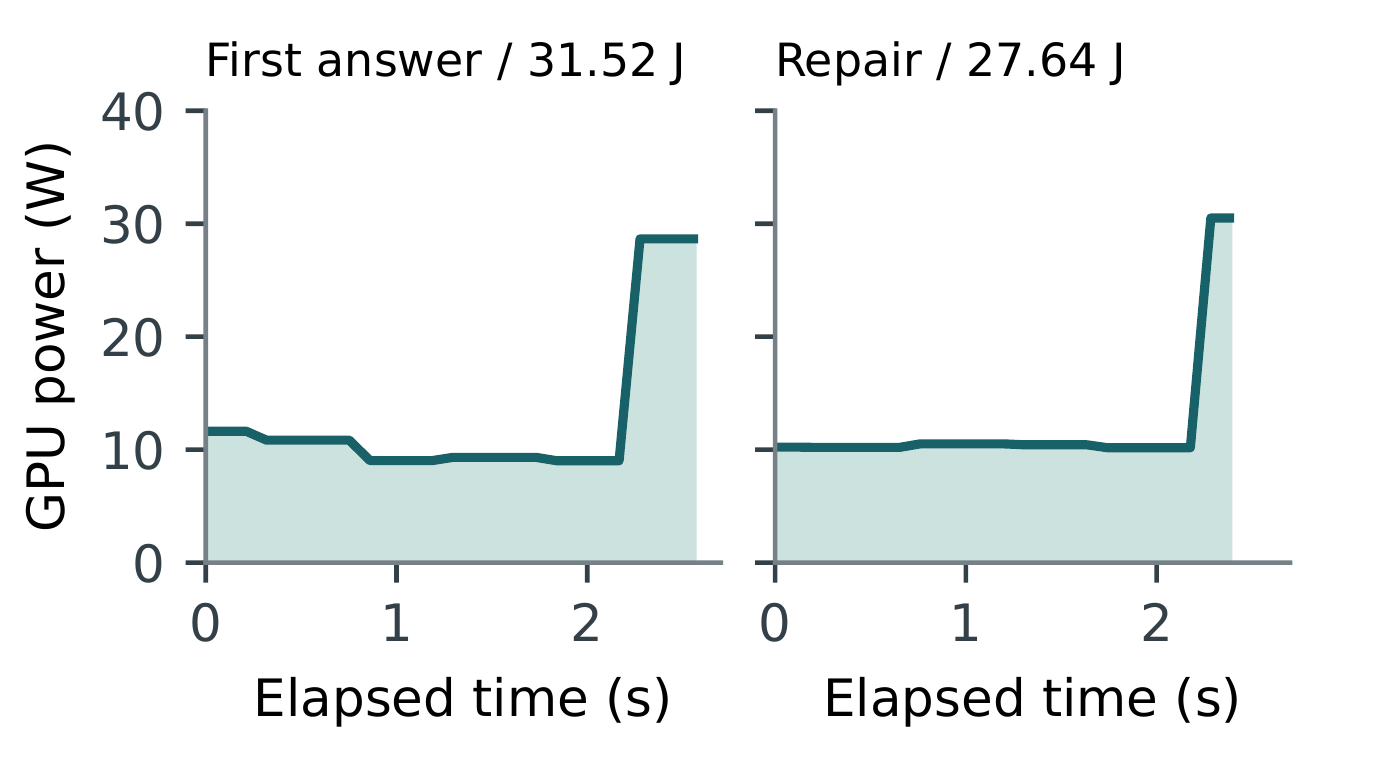
\includegraphics[width=0.78\textwidth]{figs/power_trace_original_crop.png}
\caption[GPU board power for the collision run]{Measured GPU board power for the two requests of the collision run (HumanEval/41, seed 11, short history). Shaded areas are the energies.}
\label{fig:trace}
\end{figure}

\begin{example}{Worked example: the collision run}
Integrating Fig.~\ref{fig:trace} gives 31.52\,J for the first answer and 27.64\,J for the repair: 59.16\,J for one correct solution. The first, failed request is part of the price of that success.

The trace also shows \emph{where} the energy goes. For about 2.2\,s the board sits near 10\,W; only at the end does it jump to about 30\,W, while the runtime reported just 0.30\,s of model computation for the repair. A plausible reading, which I have not separately tested, is that most of the measured energy is background board draw during the request's fixed overhead rather than model computation; the cache probe (\S2.1) shows a similar overhead. This is why subtracting an estimated idle level gave $-2.82$\,J for this short request: the idle reference exceeded the window's average draw. I report \emph{gross} board energy throughout.
\end{example}

\subsection{What the sensor does and does not see}
NVIDIA's \texttt{nvidia-smi} tool exposes both an instantaneous board power reading and a one-second average; I logged the instantaneous field about every 100\,ms. An on-board sensor is convenient but is not a calibrated instrument, and I did not calibrate my laptop's sensor against an external meter. Table~\ref{tab:boundary} states what my numbers include.

\begin{table}[h]
\centering\small
\caption{Measurement boundary of this report.}
\label{tab:boundary}
\begin{tabularx}{\columnwidth}{@{}lcY@{}}
\toprule
Component & In? & Note\\\midrule
GPU board during requests & yes & sampled $\approx$100\,ms\\
CPU running tests, RAM & no & a policy with many tests can shift energy here\\
Idle time between requests & no & \\
Power supply losses (wall) & no & needs a plug-in meter\\
Hardware manufacture & no & lifecycle (embodied) share\\\bottomrule
\end{tabularx}
\end{table}

\subsection{A fair metric: energy per correct solution}
Let $y_i=1$ if run $i$'s submitted program passes both test suites. For $N$ runs of a policy, its success rate and mean energy per run are $\hat p=\frac1N\sum_i y_i$ and $\bar E=\frac1N\sum_i E_i$. I charge all energy, including failed runs, to the successes:
\begin{equation}
J=\frac{\sum_i E_i}{\sum_i y_i}=\frac{\bar E}{\hat p}\qquad(\hat p>0).
\end{equation}
For two policies $A$ and $B$, rearranging gives a simple \textbf{break-even test}:
\begin{equation}
J_B<J_A\iff \frac{\bar E_B}{\bar E_A}<\frac{\hat p_B}{\hat p_A}.
\end{equation}
In words: \emph{if repair adds 10\% to the energy of a run, it must raise the success rate by more than 10\% (relative) to lower the energy per correct solution.} A team that values each extra correct answer highly may still choose repair; Eq.~(5) tells them what that choice costs.

\subsection{From energy to emissions}
Operational emissions multiply electricity $W_t$ (kWh) in each period $t$ by that period's grid intensity $g_t$ (kg\,CO$_2$e/kWh):
\begin{equation}
M_{\mathrm{op}}=\textstyle\sum_t W_t\,g_t .
\end{equation}
It is most useful as a \emph{rate} per unit of useful work; for an agent, ``one correct solution'' is a natural unit. For Indian deployments, grid factors are published in the Central Electricity Authority's CO$_2$ Baseline Database~\cite{cea_co2}.

\begin{example}{Illustration (national average intensity)}
My 72 short-history runs used 11.11\,kJ $=$ 3.09\,Wh of GPU board energy. The CEA database gives an all-India weighted average of 0.675\,t\,CO$_2$/MWh ($=$0.675\,kg/kWh) for FY 2025--26~\cite{cea_co2}. Multiplying, the batch corresponds to about 2.1\,g CO$_2$. This is a national annual average, not the grid mix where and when my runs happened, and it excludes the CPU, the rest of the laptop and manufacturing. Tiny for one batch, but it scales with volume. Also, efficiency per answer is not the same as total impact: if a service cuts energy per job by 20\% and then serves 50\% more jobs, its total use becomes $0.8\times1.5=1.2$ times the original.
\end{example}

% =====================================================================
\section{Case study 1: a pilot on a laptop GPU}
\subsection{Setup}
I prepared the pipeline on eight development problems, then evaluated 24 held-out HumanEval problems~\cite{chen2021humaneval}. I ran the open-weight model Qwen2.5-Coder 7B (Q4\_K\_M) locally on an RTX~5070 Laptop GPU, with temperature 0.2, an 8{,}192-token context and a 1{,}024-token output cap. Original HumanEval tests gave the visible feedback; EvalPlus tests~\cite{liu2023evalplus} were scored after each run in a sandbox with a 30-second limit per test program. I compared three policies:
\begin{itemize}
\item \textbf{One attempt:} submit the first program.
\item \textbf{Full history:} on failure, append the previous answer and failure message to the conversation.
\item \textbf{Short history:} on failure, send only the task, the latest code and the latest failure message.
\end{itemize}
Repair policies stopped at the first visible pass or after four attempts, and the final candidate was scored. Every policy ran on every problem with seeds 11, 29 and 47 (the seed advanced by one per repair), in shuffled order: $24\times3\times3=216$ runs and 259 requests. Code, prompts, raw power logs and analysis scripts are in my repository (\S\ref{sec:code}).

\subsection{Results}
\begin{table}[h]
\centering\small
\caption[Outcomes over 72 runs per policy]{Outcomes over 72 runs per policy (GPU energy of inference requests; the last column includes energy spent on failures).}
\label{tab:main}
\begin{tabular}{@{}lcccc@{}}
\toprule
Policy & Correct & Success & J/run & J/correct\\\midrule
One attempt & 60/72 & 83.3\% & 107.09 & \textbf{128.51}\\
Full history & 62/72 & 86.1\% & 163.00 & 189.29\\
Short history & 63/72 & 87.5\% & 154.36 & 176.41\\\bottomrule
\end{tabular}
\end{table}

\begin{figure}[t]
\centering
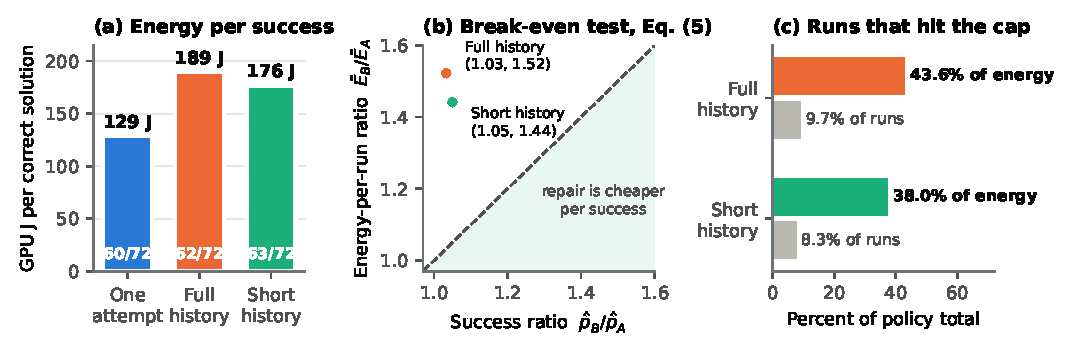
\includegraphics[width=\textwidth]{figs/results.pdf}
\caption[Energy per correct solution, break-even test, cap-hit share]{(a) One attempt used the least GPU energy per correct solution. (b) The break-even test of Eq.~(5): each repair policy is plotted against one attempt; points above the dashed line cost more energy per success, and both lie far above it. (c) Runs that reached the four-attempt cap were a small share of runs but a large share of energy, and none of them succeeded.}
\label{fig:results}
\end{figure}

\textbf{Repair raised accuracy a little and energy a lot.} Energy per run rose by 52\% (full) and 44\% (short), while success rose by only 3\% and 5\% in relative terms. By Eq.~(5), the gain is far too small to pay for the energy (Fig.~\ref{fig:results}b). Requests per policy grew less than energy: 72, 95 and 92 requests, so mean energy per request rose from 107\,J to 124\,J (full) and 121\,J (short). Revision requests carry longer prompts than first attempts.

\textbf{What repair actually bought.} Repair rescued exactly two failed first answers in each repair policy. Full history's entire net gain over one attempt came from a single problem, the collision example, and one of short history's three extra successes came from a different \emph{first} answer rather than from repair: even with matched seeds, the two repair policies produced different first programs in 6 of 72 pairs before any feedback was given.

\textbf{Where the extra energy went.} Most runs ended after one attempt. All 13 runs that reached the four-attempt cap failed, yet they consumed 44\% (full) and 38\% (short) of their policies' energy (Fig.~\ref{fig:results}c). In hindsight a two-attempt cap would have kept every rescue, but reaching the cap selects the hardest problems, so a cap must be tested on fresh data.

\textbf{How certain?} Resampling the 24 problems 10{,}000 times, the energy-per-success ratios against one attempt (1.47 for full and 1.37 for short history) both had 95\% intervals entirely above 1. Short versus full history ($0.93$, interval $[0.82,\,1.08]$) was unresolved, and only 17 runs entered repair at all. Because each policy also had its own first answer, the pilot could not separate repair from first-answer variation. These gaps motivated the second case study.

% =====================================================================
\section{Case study 2: answering the open questions}\label{sec:followup}
The pilot left three questions open: whether short or full history is better, whether a stop on lack of progress keeps the rescues, and whether the answer changes with model size. Its design could not settle them, because each policy produced its own first answer. I therefore ran a second experiment designed to answer exactly these questions.

\subsection{Design}
\textbf{Same failure, many continuations.} For every run, the model first answers once. If that answer fails a visible check, three continuations start from the \emph{same} failed program: \emph{full history} (the conversation grows), \emph{short history} (task, latest code, latest failure) and a \emph{fresh retry} (the original prompt again, with a new seed and no feedback). Each continuation runs to a visible pass or four attempts. Every stopping policy is then read off these recorded trajectories, so all policies are compared on identical cases and charged for the same first request.

\textbf{The progress-based stop.} Let $v_t$ be the number of visible checks passed by attempt $t$ and $b_t=\max_{s\le t}v_s$ the best so far. A counter resets when $v_t>b_{t-1}$ and grows by one otherwise. The rule submits on a visible pass, stops when the counter reaches the patience $K$ or at four attempts, and on a non-accepting stop returns the \emph{earliest} attempt that reached $b_t$. To make this possible, the harness splits each problem's test into separate checks and records every one.

\textbf{Problems and models.} I used the 140 HumanEval problems not used in the pilot~\cite{chen2021humaneval}, so no problem was seen while designing the policies. Two models from the same family ran on the laptop GPU through Ollama 0.40.16: Qwen2.5-Coder 1.5B and 7B, both quantized to Q4\_K\_M, with the pilot's settings. The 1.5B model ran every problem with seed 11; the 7B model ran every problem with seed 11 and 103 further runs with seeds 29 and 47. In total there were 383 runs and 1{,}128 model requests, each matched to at least 18 power samples. Hidden EvalPlus tests~\cite{liu2023evalplus} decided correctness, and intervals come from a bootstrap that resamples whole problems 10{,}000 times.

\begin{table}[h]
\centering\small
\caption[Follow-up: success and energy per correct solution]{Follow-up results. Success and GPU energy per correct solution (J) for each policy. Rescues count failed first answers turned into correct submissions.}
\label{tab:followup}
\begin{tabular}{@{}lcccccc@{}}
\toprule
& \multicolumn{3}{c}{Qwen2.5-Coder 1.5B (140 runs)} & \multicolumn{3}{c}{Qwen2.5-Coder 7B (243 runs)}\\
\cmidrule(lr){2-4}\cmidrule(l){5-7}
Policy & Success & J/correct & Rescues & Success & J/correct & Rescues\\\midrule
One attempt & 66.4\% & \textbf{109} & -- & 77.0\% & \textbf{227} & --\\
Full history, cap 4 & 67.9\% & 204 & 2 & 77.4\% & 372 & 1\\
Short history, cap 4 & 67.1\% & 206 & 1 & 78.6\% & 364 & 4\\
Fresh retry, cap 2 & 70.0\% & 137 & 5 & 78.2\% & 272 & 3\\
Fresh retry, cap 4 & \textbf{75.0\%} & 179 & 12 & \textbf{80.2\%} & 345 & 8\\
Short history, progress stop $K{=}1$ & 67.1\% & 142 & 1 & 77.8\% & 278 & 2\\\midrule
Failed first answers & \multicolumn{3}{c}{42} & \multicolumn{3}{c}{46}\\\bottomrule
\end{tabular}
\end{table}

\begin{figure}[t]
\centering
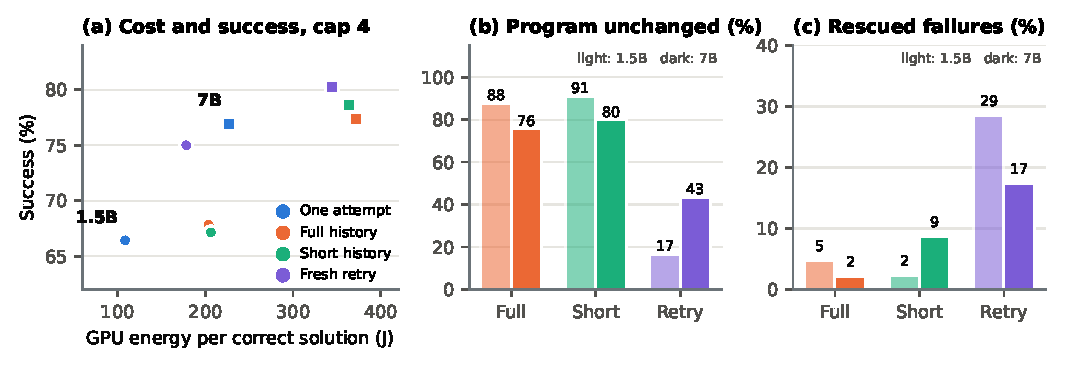
\includegraphics[width=\textwidth]{figs/followup.pdf}
\caption[Follow-up: cost against success, unchanged resubmissions and rescues]{(a) Success against GPU energy per correct solution at a four-attempt cap; circles are the 1.5B model, squares the 7B model. (b) Share of continuation attempts that returned exactly the program of the previous attempt. (c) Share of failed first answers that each continuation turned into a correct submission.}
\label{fig:followup}
\end{figure}

\subsection{Short or full history?}
\textbf{Neither, measurably.} At a four-attempt cap, short history cost $0.98\times$ the energy per correct solution of full history for the 7B model (95\% interval $[0.94,\,1.01]$) and $1.01\times$ for the 1.5B model ($[0.98,\,1.06]$). Success differed by at most 1.2 points. The pilot's open question has a clear answer: on these tasks, the amount of history does not matter.

\textbf{Why: the model repeats itself.} Fig.~\ref{fig:followup}b shows the reason. After seeing its failure, the model returned an \emph{unchanged} program in 76\% (full) and 80\% (short) of the 7B model's repair attempts, and in 88\% and 91\% of the 1.5B model's. An unchanged program fails the same check again, so most repair requests bought nothing. This matches Olausson et al.'s finding that repair is limited by the quality of the model's feedback on its own code~\cite{olausson2024selfrepair}.

\textbf{A fresh retry did better.} Re-asking the original question without any feedback changed the program far more often and rescued far more failures: 12 of 42 for the 1.5B model and 8 of 46 for the 7B model, against at most 4 for either repair style (Fig.~\ref{fig:followup}c). For the 1.5B model, a fresh retry beat short history by 7.9 points of success (interval $[3.6,\,12.9]$) at $0.87\times$ the energy per correct solution ($[0.77,\,0.95]$). For the 7B model the same direction holds, but the intervals include no difference. In the language of \S\ref{sec:pk}, independent samples were more useful than feedback-driven revisions here: the feedback anchored the model on its own wrong answer.

\textbf{Still not free.} Every multi-attempt policy cost more energy per correct solution than one attempt; even the best one, a fresh retry with cap 4, cost $1.52\times$ ($[1.32,\,1.73]$) for the 7B model and $1.64\times$ ($[1.44,\,1.86]$) for the 1.5B model. Retrying buys accuracy, not efficiency.

\subsection{Does a progress-based stop keep the rescues?}
\textbf{For repair, yes; but a fixed cap does as well.} With patience $K=1$, the progress stop gave up no rescues of full history for either model and two of the 7B model's four short-history rescues, while cutting energy per correct solution by a quarter to a third relative to a four-attempt cap (short history, 7B: $0.76\times$, interval $[0.71,\,0.84]$). Because repairs so often repeated the same program, the counter almost always stopped after the second attempt, so the rule behaved like a two-attempt cap and saved the same energy.

\textbf{For a fresh retry, visible progress is the wrong signal.} Retries are independent, so a retry that passes fewer checks says little about the next one. With $K=1$, the rule gave up 5 of the 12 retry rescues of the 1.5B model and 5 of the 8 of the 7B model; with $K=2$ it gave up one in each, for about a tenth less energy than cap 4. A fixed budget of attempts is the simpler and safer rule for retries.

\subsection{Does the answer change with model size?}
On the 140 problems both models ran with seed 11, the 7B model's single attempt succeeded on 79.3\% against 66.4\% for the 1.5B model, a gap of 12.9 points (interval $[5.7,\,20.0]$), but it used about twice the energy per correct solution: the 1.5B model needed $0.51\times$ as much ($[0.45,\,0.57]$). Each generated token cost about 1.04\,J on the 7B model and 0.46\,J on the 1.5B model.

Spending the saving on retries narrows the gap. The 1.5B model with up to four fresh retries reached 75.0\%, 4.3 points below the 7B model's single attempt (interval $[-11.4,\,+2.9]$), at $0.83\times$ its energy per correct solution ($[0.69,\,1.01]$). Neither difference is statistically clear, so I do not claim the small model is better. The design point is still useful: a smaller model that retries is a serious alternative to a larger model that answers once, and the choice should be measured rather than assumed.

\textbf{What no policy can fix.} Some first answers passed every visible check but failed the hidden tests: 5 of the 1.5B model's 140 and 6 of the 7B model's 140 seed-11 runs. Every policy accepts these at once, so their errors are invisible to the loop. Better verifiers, not more attempts, are the remedy.

% =====================================================================
\section{From a laptop to production and repository scale}\label{sec:production}
\subsection{A production model on the same problems}
Production models differ from local ones in size, hardware and in how they generate: many now produce hidden ``thinking'' tokens before the visible answer. To see what this means for the same question, I ran the identical harness against Google's Gemini 3 Flash (\texttt{gemini-3-flash-preview}) through the Gemini API. The free tier allowed only 11 of the 140 problems in one day, so these results are \emph{preliminary}.

On those 11 problems, Gemini's first attempt was correct on 10, against 9 for the 7B model and 8 for the 1.5B model. The sample is far too small to rank the models. The token counts are more informative. Gemini's visible answers were similar in length to the local models' (median 207 output tokens, against 144--147), but before answering it generated hidden reasoning tokens: a median of 1{,}224 and a mean of about 4{,}000 per first request. In 6 of the 11 first requests the reasoning stopped at about 7{,}860 tokens, apparently at the limit implied by my 8{,}192-token output cap, so these counts are lower bounds. By the mean, the production model generated about 29 times as many tokens per answer as the local models; by the median, about 10 times. The one failed problem (HumanEval/141) also shows the cost of retrying such a model: six of its seven continuation requests reached the token cap, and the only visible pass, from full history, still failed the hidden tests.

\textbf{Energy.} I cannot measure the energy of a hosted model. The best public reference is Google's own measurement of its Gemini Apps service: the median text prompt used 0.24\,Wh with a comprehensive boundary that includes host machines, idle capacity and data-centre overhead, and 0.10\,Wh when counting only active AI accelerators~\cite{google2025gemini}. The accelerator-only figure, about 360\,J, is the closest match to my GPU-board boundary. My laptop's median first request used 152\,J (7B) and 69\,J (1.5B). These numbers are the same order of magnitude, but they are not a like-for-like comparison: Google's figure is a median over a different mix of prompts and models, and a request with thousands of reasoning tokens may sit well above the median.

\begin{keybox}{What changes in production}
\textbf{Retries are cheap to buy and expensive in total.} An API user pays per token, not per joule, and never sees the energy. A model that thinks for thousands of tokens makes every extra attempt costly, so the stopping rule matters at least as much as on a laptop.

\textbf{Accuracy headroom is smaller.} A strong model fails less often, so fewer runs reach a retry at all, and the expected value of an extra attempt falls with the failure rate.

\textbf{Scale multiplies small savings.} A stopping rule that saves a quarter of the energy on failed runs is negligible for one user and material for a service answering millions of requests a day.
\end{keybox}

\subsection{At repository scale: SWE-bench}
HumanEval asks for one function. SWE-bench asks an agent to resolve a real GitHub issue in a full repository: find the right file, read tests, edit, and check that nothing else broke. A file read can be essential to a later fix without changing any test result, so ``tests passed so far'' is a weaker progress signal at this scale.

I compared two public SWE-bench Verified submissions on the same 500 tasks~\cite{swebench_exp}. Their metadata list them as mini-SWE-agent v2.0.0 runs with GPT-5.2 Codex (19 February 2026) and Gemini 3 Pro (26 February 2026). The per-task evaluator records I used give 364 and 353 successes; the summary metadata give 364 and 348. Because the second pair disagrees, I treat the comparison as one between archived submissions.

\begin{table}[h]
\centering\small
\caption[SWE-bench: per-task outcomes of two snapshots]{Per-task outcomes of the two snapshots.}
\label{tab:swe}
\begin{tabular}{@{}lcc@{}}
\toprule
& Second solved & Second failed\\\midrule
First solved & 320 & 44\\
First failed & 33 & 103\\\bottomrule
\end{tabular}
\end{table}

The totals differ by only 11, but the snapshots disagree on 77 tasks (Table~\ref{tab:swe}). An oracle that always picked the right submission would solve $320+44+33=397$. This is hindsight: a real selector must decide from evidence available before grading, and pay for the second run. A paired task bootstrap puts the difference in success rates ($-2.2$ points) between about $-5.6$ and $+1.2$ points, so 500 tasks cannot separate the two overall rates.

Cost differs more clearly than accuracy: the submissions' metadata report means of 28.1 and 51.3 model calls per task. Energy cannot be estimated from public data at all. At this scale, the lesson of my experiments still applies but is harder to act on: a stopping rule needs a progress signal, and ``tests passed so far'' is a weak one when most steps are reading and searching.

% =====================================================================
\section{Policy: telling users why the agent stopped}
India's Ministry of Electronics and Information Technology released the India AI Governance Guidelines on 5 November 2025~\cite{meity2025}. They are principle-based: seven ``sutras'' include \emph{Accountability}, \emph{Understandable by Design}, and \emph{Safety, Resilience \& Sustainability}. The guidelines do not prescribe energy logs. Applying their principles to a stopping agent, I propose the record in Table~\ref{tab:card}.

\begin{table}[h]
\centering\small
\caption[Proposed per-answer disclosure]{Proposed per-answer disclosure, filled in for the collision run.}
\label{tab:card}
\begin{tabularx}{\columnwidth}{@{}lY@{}}
\toprule
Field & Collision run (HumanEval/41)\\\midrule
Stopping reason & visible test passed\\
Attempts used & 2 of 4\\
Checks visible to agent & example $n=2\to4$\\
Energy and boundary & 59.16\,J, GPU board, inference only\\
Hidden-test result & passed (evaluation only; unknown at deployment)\\\bottomrule
\end{tabularx}
\end{table}

A run that stops because its budget ran out should instead list which checks still fail. The two reasons call for different levels of human review. For a batch, I would add the model and hardware, total jobs, successful submissions and total measured energy. For a hosted model, whose energy the user cannot observe, the record should instead give token counts, \emph{including hidden reasoning tokens}: Section~\ref{sec:production} showed that these can outnumber the visible answer many times over.

% =====================================================================
\section{Limitations}
\begin{itemize}
\item \textbf{One task family.} Single-function Python problems with prompts under about 2{,}000 tokens; repository-scale agents were studied only through archived public submissions, without energy.
\item \textbf{Two small local models.} Both from one family, 4-bit quantized, on one laptop GPU; the size comparison rests on one seed per model.
\item \textbf{Partial energy boundary.} GPU board power only, from an uncalibrated sensor; CPU, memory, the rest of the laptop and manufacturing are excluded. While the Gemini run tested its programs on the CPU, the 7B run shared the machine; this should barely affect GPU board power.
\item \textbf{Production model.} Only 11 problems on a free tier, with an output cap that limited the model's reasoning; its energy is a published median for a different workload, not a measurement.
\item \textbf{Low temperature.} At temperature 0.2, retries are less diverse than at higher settings; the advantage of fresh retries may change with sampling settings.
\end{itemize}

\section{Conclusion}
Measured as energy per correct solution, every extra attempt cost more than it returned: one attempt was the most efficient policy in the pilot and for both model sizes in the follow-up. When accuracy matters more than energy, \emph{how} the extra attempt is spent matters more than whether it is spent. Feeding the failure back was mostly wasted, because the model resubmitted the same program, while a fresh attempt from the original prompt rescued up to a third of the failures. Whether to take another step therefore depends on the two quantities the foundations made precise: how informative the feedback is, and whether the extra success clears the break-even condition of Eq.~(5).

\begin{keybox}{What this study answers, and what it does not}
\textbf{Answers.} On HumanEval with local Qwen2.5-Coder models: one attempt gives the lowest GPU energy per correct solution. Short and full history perform the same, because the model mostly repeats its program after feedback. A fresh retry rescues far more failures than either repair style. A progress-based stop keeps nearly all repair rescues at a quarter to a third less energy than a four-attempt cap, but it is no better than a two-attempt cap and should not be used for retries. A 1.5B model with retries comes within a statistically unclear 4 points of a 7B model's single attempt at lower energy.

\textbf{Does not answer.} The energy of production models, which only their operators can measure; how these results transfer to repository-scale agents, where progress is harder to observe; and whole-system energy beyond the GPU board. The production run is preliminary and should be extended to all 140 problems.
\end{keybox}

\section{Code and data availability}\label{sec:code}
All code, prompts, raw power traces, run logs, hidden-test scores, and the analysis and plotting scripts for both case studies and the production run are available at \repourl. The follow-up data are in \texttt{data/followup/} and the scripts in \texttt{experiment2/}; every number in Sections~\ref{sec:followup} and \ref{sec:production} can be regenerated from them.

\bibliographystyle{unsrt}
\bibliography{refs}

\end{document}
